\chapter{Controlador}

Este capítulo descreve o Controlador. Este é um software projetado para controlar a simulação garantindo sincronia com o Gazebo. Inicialmente, é descrito a localização de seus componente no projeto e a arquitetura de software utilizada.e seus arquivos de configuração. Em seguida, será exposto como é realizado a sua configuração e o processo de comunicação com os plugins do Gazebo. Por fim, é especificado os plugins de controle existentes, o processo de criação de novos plugins de controle e o processo de armazenamento de dados de simulação.

\section{Localização no projeto}


\textbf{\emph{Controller}}
\vspace{0.5em}

A figura \ref{fig:arvore_controller} ilustra o diretório \emph{Controller}.

\begin{tiny}
	\begin{figure}[htbp]
		\begin{forest}
			for tree={font=\sffamily, grow'=0,
				folder indent=.9em, folder icons,
				edge=densely dotted}
			[Controller
			[include
			]
			[src
			]
			[CMakeLists.txt
			]
			[package.xml
			]
			]
		\end{forest}
		\caption{Árvore do diretório \emph{Controller}.}
		\label{fig:arvore_controller}
	\end{figure}
\end{tiny}

\vspace{0.5em}
\noindent 
\textbf{\emph{control\_strategies}}
\vspace{0.5em}

A figura \ref{fig:arvore_control} ilustra o diretório \emph{control\_strategies}.

\begin{tiny}
	\begin{figure}[htbp]
		\begin{forest}
			for tree={font=\sffamily, grow'=0,
				folder indent=.9em, folder icons,
				edge=densely dotted}
			[control\_strategies
			[vant2load\_hinfinity
			]
			[vant2\_lqr
			]
			[vant3\_adaptiveMixCtrl
			]
			[vant3\_lqr
			]
			[vantloadMarcelo
			]
			[lcontroller.hpp, is file]
			]
		\end{forest}
		\caption{Árvore do diretório \emph{control\_strategies}.}
		\label{fig:arvore_control}
	\end{figure}
\end{tiny}

\vspace{0.5em}
\noindent 
\textbf{\emph{custom\_plugins}}
\vspace{0.5em}

A figura \ref{fig:arvore_customplugins} ilustra o diretório \emph{custom\_plugins}.

\begin{tiny}
	\begin{figure}[htbp]
		\begin{forest}
			for tree={font=\sffamily, grow'=0,
				folder indent=.9em, folder icons,
				edge=densely dotted}
			[custom\_plugins
			[include
			]
			[src
			]
			[plugins
			]
			[CMakeLists.txt
			]
			[package.xml
			]
			]
		\end{forest}
		\caption{Árvore do diretório \emph{custom\_plugins}.}
		\label{fig:arvore_customplugins}
	\end{figure}
\end{tiny}

\vspace{0.5em}
\noindent 
\textbf{\emph{Matlab}}
\vspace{0.5em}

A figura \ref{fig:arvore_matlab} ilustra o diretório \emph{Matlab}.

\begin{tiny}
	\begin{figure}[htbp]
		\begin{forest}
			for tree={font=\sffamily, grow'=0,
				folder indent=.9em, folder icons,
				edge=densely dotted}
			[Matlab
			[erro.txt, is file]
			[in.txt, is file]
			[out.txt, is file]
			[ref.txt, is file]
			]
		\end{forest}
		\caption{Árvore do diretório \emph{Matlab}.}
		\label{fig:arvore_matlab}
	\end{figure}
\end{tiny}

\vspace{0.5em}
\noindent 
\textbf{\emph{simulator\_msgs}}
\vspace{0.5em}

A figura \ref{fig:arvore_matlab} ilustra o diretório \emph{Matlab}.

\begin{tiny}
	\begin{figure}[htbp]
		\begin{forest}
			for tree={font=\sffamily, grow'=0,
				folder indent=.9em, folder icons,
				edge=densely dotted}
			[Matlab
			[msg]
			[CMakeLists.txt, is file]
			[package.xml, is file]
			]
		\end{forest}
		\caption{Árvore do diretório \emph{simulador\_msgs}.}
		\label{fig:arvore_simuladormsgs}
	\end{figure}
\end{tiny}

\section{Arquivo config.xml}

\label{config}



\section{Arquitetura de Software}


\subsection{Tópicos e mensagens do ROS entre Controlador e Sensores/Plugins}

Sensores/plugins com função sensorial comunicam com o Gazebo através de tópicos com mensagens padronizadas denominadas \textit{Sensor}. Como estas mensagens podem chegar com ordens indefinidas, existe uma lógica no controlador que ordena uma estrtura denominada SensorArray de acordo com uma ordem previamente estabelecida pelo usuário através de um arquivo XML. Assim, quando o usuário projetar um novo controlador, ele terá acesso a um vetor de sensores conforme desejado. Isto está ilustrado na Figura \ref{Msgs1.jpg}.


\begin{figure}[H]
	\centering
	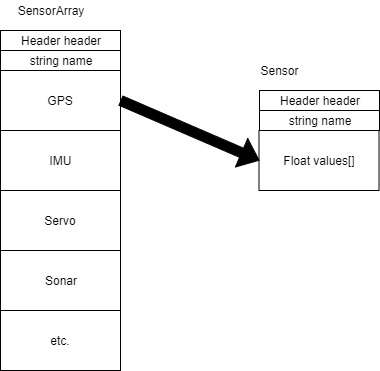
\includegraphics[width=0.65\textwidth]{figuras/Msgs1.jpg}
	\caption{Mensagens utilizadas para comunicação entre Gazebo e Simulador}
	\label{Msgs1.jpg}
\end{figure}

Além disso, a comunicação entre controlador e plugins ocorre por meio de tópicos com mensagens correspondendo a pontos flutuantes valores. Mais detalhes, o código se encontra auto-explicativo.  


\chapter{Interface Gráfica}

\section{Localização no projeto}

\section{Arquitetura de Software}


